\documentclass[a4paper]{article}

\def\npart {IV}
\def\nterm {Lent}
\def\nyear {2018}
\def\nlecturer {A.\ J.\ Scholl}
\def\ncourse {Topics in Number Theory}

% Imports
\ifx \nextra \undefined
  \usepackage[pdftex,
    hidelinks,
    pdfauthor={Dexter Chua},
    pdfsubject={Cambridge Maths Notes: Part \npart\ - \ncourse},
    pdftitle={Part \npart\ - \ncourse},
  pdfkeywords={Cambridge Mathematics Maths Math \npart\ \nterm\ \nyear\ \ncourse}]{hyperref}
  \title{Part \npart\ - \ncourse}
\else
  \usepackage[pdftex,
    hidelinks,
    pdfauthor={Dexter Chua},
    pdfsubject={Cambridge Maths Notes: Part \npart\ - \ncourse\ (\nextra)},
    pdftitle={Part \npart\ - \ncourse\ (\nextra)},
  pdfkeywords={Cambridge Mathematics Maths Math \npart\ \nterm\ \nyear\ \ncourse\ \nextra}]{hyperref}

  \title{Part \npart\ - \ncourse \\ {\Large \nextra}}
\fi

\author{Lectured by \nlecturer \\\small Notes taken by Dexter Chua}
\date{\nterm\ \nyear}

\usepackage{alltt}
\usepackage{amsfonts}
\usepackage{amsmath}
\usepackage{amssymb}
\usepackage{amsthm}
\usepackage{booktabs}
\usepackage{caption}
\usepackage{enumitem}
\usepackage{fancyhdr}
\usepackage{graphicx}
\usepackage{mathtools}
\usepackage{microtype}
\usepackage{multirow}
\usepackage{pdflscape}
\usepackage{pgfplots}
\usepackage{siunitx}
\usepackage{tabularx}
\usepackage{tikz}
\usepackage{tkz-euclide}
\usepackage[normalem]{ulem}
\usepackage[all]{xy}

\pgfplotsset{compat=1.12}

\pagestyle{fancyplain}
\lhead{\emph{\nouppercase{\leftmark}}}
\ifx \nextra \undefined
  \rhead{
    \ifnum\thepage=1
    \else
      \npart\ \ncourse
    \fi}
\else
  \rhead{
    \ifnum\thepage=1
    \else
      \npart\ \ncourse\ (\nextra)
    \fi}
\fi
\usetikzlibrary{arrows}
\usetikzlibrary{decorations.markings}
\usetikzlibrary{decorations.pathmorphing}
\usetikzlibrary{positioning}
\usetikzlibrary{fadings}
\usetikzlibrary{intersections}
\usetikzlibrary{cd}

\newcommand*{\Cdot}{\raisebox{-0.25ex}{\scalebox{1.5}{$\cdot$}}}
\newcommand {\pd}[2][ ]{
  \ifx #1 { }
    \frac{\partial}{\partial #2}
  \else
    \frac{\partial^{#1}}{\partial #2^{#1}}
  \fi
}

% Theorems
\theoremstyle{definition}
\newtheorem*{aim}{Aim}
\newtheorem*{axiom}{Axiom}
\newtheorem*{claim}{Claim}
\newtheorem*{cor}{Corollary}
\newtheorem*{defi}{Definition}
\newtheorem*{eg}{Example}
\newtheorem*{fact}{Fact}
\newtheorem*{law}{Law}
\newtheorem*{lemma}{Lemma}
\newtheorem*{notation}{Notation}
\newtheorem*{prop}{Proposition}
\newtheorem*{thm}{Theorem}

\renewcommand{\labelitemi}{--}
\renewcommand{\labelitemii}{$\circ$}
\renewcommand{\labelenumi}{(\roman{*})}

\let\stdsection\section
\renewcommand\section{\newpage\stdsection}

% Strike through
\def\st{\bgroup \ULdepth=-.55ex \ULset}

% Maths symbols
\newcommand{\bra}{\langle}
\newcommand{\ket}{\rangle}

\newcommand{\N}{\mathbb{N}}
\newcommand{\Z}{\mathbb{Z}}
\newcommand{\Q}{\mathbb{Q}}
\renewcommand{\H}{\mathbb{H}}
\newcommand{\R}{\mathbb{R}}
\newcommand{\C}{\mathbb{C}}
\newcommand{\Prob}{\mathbb{P}}
\renewcommand{\P}{\mathbb{P}}
\newcommand{\E}{\mathbb{E}}
\newcommand{\F}{\mathbb{F}}
\newcommand{\cU}{\mathcal{U}}
\newcommand{\RP}{\mathbb{RP}}
\newcommand{\CP}{\mathbb{CP}}

\newcommand{\ph}{\,\cdot\,}

\DeclareMathOperator{\sech}{sech}
\DeclareMathOperator{\cosech}{cosech}
\DeclareMathOperator{\cosec}{cosec}

\DeclareMathOperator{\covol}{covol}
\DeclareMathOperator{\vol}{vol}

\let\Im\relax
\let\Re\relax
\DeclareMathOperator{\Im}{Im}
\DeclareMathOperator{\Re}{Re}
\DeclareMathOperator{\im}{im}
\DeclareMathOperator{\image}{image}
\DeclareMathOperator{\Ann}{Ann}

\DeclareMathOperator*{\res}{res}
\DeclareMathOperator{\Res}{Res}
\DeclareMathOperator{\Ind}{Ind}

\DeclareMathOperator{\tr}{tr}
\DeclareMathOperator{\diag}{diag}
\DeclareMathOperator{\rank}{rank}
\DeclareMathOperator{\card}{card}
\DeclareMathOperator{\spn}{span}
\DeclareMathOperator{\adj}{adj}

\DeclareMathOperator{\erf}{erf}
\DeclareMathOperator{\erfc}{erfc}

\DeclareMathOperator{\ord}{ord}
\DeclareMathOperator{\Sym}{Sym}

\DeclareMathOperator{\sgn}{sgn}
\DeclareMathOperator{\orb}{orb}
\DeclareMathOperator{\stab}{stab}
\DeclareMathOperator{\ccl}{ccl}

\DeclareMathOperator{\lcm}{lcm}
\DeclareMathOperator{\hcf}{hcf}

\DeclareMathOperator{\Int}{Int}
\DeclareMathOperator{\id}{id}

\DeclareMathOperator{\betaD}{beta}
\DeclareMathOperator{\gammaD}{gamma}
\DeclareMathOperator{\Poisson}{Poisson}
\DeclareMathOperator{\binomial}{binomial}
\DeclareMathOperator{\multinomial}{multinomial}
\DeclareMathOperator{\Bernoulli}{Bernoulli}
\DeclareMathOperator{\like}{like}

\DeclareMathOperator{\var}{var}
\DeclareMathOperator{\cov}{cov}
\DeclareMathOperator{\bias}{bias}
\DeclareMathOperator{\mse}{mse}
\DeclareMathOperator{\corr}{corr}

\DeclareMathOperator{\otp}{otp}
\DeclareMathOperator{\dom}{dom}

\DeclareMathOperator{\Root}{Root}
\DeclareMathOperator{\supp}{supp}
\DeclareMathOperator{\rel}{rel}
\DeclareMathOperator{\Hom}{Hom}
\DeclareMathOperator{\Aut}{Aut}
\DeclareMathOperator{\Gal}{Gal}
\DeclareMathOperator{\Mat}{Mat}
\DeclareMathOperator{\End}{End}
\DeclareMathOperator{\Char}{char}
\DeclareMathOperator{\ev}{ev}
\DeclareMathOperator{\St}{St}
\DeclareMathOperator{\Lk}{Lk}
\DeclareMathOperator{\disc}{disc}
\DeclareMathOperator{\Isom}{Isom}
\DeclareMathOperator{\length}{length}
\DeclareMathOperator{\energy}{energy}
\DeclareMathOperator{\area}{area}
\DeclareMathOperator{\Syl}{Syl}
\DeclareMathOperator{\cl}{cl}
\DeclareMathOperator{\fix}{fix}

\newcommand{\GL}{\mathrm{GL}}
\newcommand{\SL}{\mathrm{SL}}
\newcommand{\PGL}{\mathrm{PGL}}
\newcommand{\PSL}{\mathrm{PSL}}
\newcommand{\PSU}{\mathrm{PSU}}
\newcommand{\Or}{\mathrm{O}}
\newcommand{\SO}{\mathrm{SO}}
\newcommand{\U}{\mathrm{U}}
\newcommand{\SU}{\mathrm{SU}}

\renewcommand{\d}{\mathrm{d}}
\newcommand{\D}{\mathrm{D}}

\tikzset{->/.style = {decoration={markings,
                                  mark=at position 1 with {\arrow[scale=2]{latex'}}},
                      postaction={decorate}}}
\tikzset{<-/.style = {decoration={markings,
                                  mark=at position 0 with {\arrowreversed[scale=2]{latex'}}},
                      postaction={decorate}}}
\tikzset{<->/.style = {decoration={markings,
                                   mark=at position 0 with {\arrowreversed[scale=2]{latex'}},
                                   mark=at position 1 with {\arrow[scale=2]{latex'}}},
                       postaction={decorate}}}
\tikzset{->-/.style = {decoration={markings,
                                   mark=at position #1 with {\arrow[scale=2]{latex'}}},
                       postaction={decorate}}}
\tikzset{-<-/.style = {decoration={markings,
                                   mark=at position #1 with {\arrowreversed[scale=2]{latex'}}},
                       postaction={decorate}}}

\tikzset{circ/.style = {fill, circle, inner sep = 0, minimum size = 3}}
\tikzset{mstate/.style={circle, draw, blue, text=black, minimum width=0.7cm}}

\definecolor{mblue}{rgb}{0.2, 0.3, 0.8}
\definecolor{morange}{rgb}{1, 0.5, 0}
\definecolor{mgreen}{rgb}{0.1, 0.4, 0.2}
\definecolor{mred}{rgb}{0.5, 0, 0}

\def\drawcirculararc(#1,#2)(#3,#4)(#5,#6){%
    \pgfmathsetmacro\cA{(#1*#1+#2*#2-#3*#3-#4*#4)/2}%
    \pgfmathsetmacro\cB{(#1*#1+#2*#2-#5*#5-#6*#6)/2}%
    \pgfmathsetmacro\cy{(\cB*(#1-#3)-\cA*(#1-#5))/%
                        ((#2-#6)*(#1-#3)-(#2-#4)*(#1-#5))}%
    \pgfmathsetmacro\cx{(\cA-\cy*(#2-#4))/(#1-#3)}%
    \pgfmathsetmacro\cr{sqrt((#1-\cx)*(#1-\cx)+(#2-\cy)*(#2-\cy))}%
    \pgfmathsetmacro\cA{atan2(#2-\cy,#1-\cx)}%
    \pgfmathsetmacro\cB{atan2(#6-\cy,#5-\cx)}%
    \pgfmathparse{\cB<\cA}%
    \ifnum\pgfmathresult=1
        \pgfmathsetmacro\cB{\cB+360}%
    \fi
    \draw (#1,#2) arc (\cA:\cB:\cr);%
}
\newcommand\getCoord[3]{\newdimen{#1}\newdimen{#2}\pgfextractx{#1}{\pgfpointanchor{#3}{center}}\pgfextracty{#2}{\pgfpointanchor{#3}{center}}}

\def\Xint#1{\mathchoice
   {\XXint\displaystyle\textstyle{#1}}%
   {\XXint\textstyle\scriptstyle{#1}}%
   {\XXint\scriptstyle\scriptscriptstyle{#1}}%
   {\XXint\scriptscriptstyle\scriptscriptstyle{#1}}%
   \!\int}
\def\XXint#1#2#3{{\setbox0=\hbox{$#1{#2#3}{\int}$}
     \vcenter{\hbox{$#2#3$}}\kern-.5\wd0}}
\def\ddashint{\Xint=}
\def\dashint{\Xint-}

\DeclareMathOperator\Br{Br}
\renewcommand\G{\mathbb{G}}
\newcommand\A{\mathbb{A}}
\DeclareMathOperator\Cl{\mathrm{Cl}}
\newcommand\ab{\mathrm{ab}}
\newcommand\sprime{\!{\vphantom{\prod}}'}

\begin{document}
\maketitle
{\small
\setlength{\parindent}{0em}
\setlength{\parskip}{1em}
The ``Langlands programme'' is a far-ranging series of conjectures describing the connections between automorphic forms on the one hand, and algebraic number theory and arithmetic algebraic geometry on the other. In these lectures we will give an introduction to some aspects of this programme.

\subsubsection*{Pre-requisites}
The course will follow on naturally from the Michaelmas term courses \emph{Algebraic Number Theory} and \emph{Modular Forms and L-Functions}, and knowledge of them will be assumed. Some knowledge of algebraic geometry will be required in places.
}
\tableofcontents

\setcounter{section}{-1}
\section{Introduction}
In this course, we shall first give an outline of class field theory. We then look at abelian $L$-functions (Hecke, Tate). We then talk about \emph{non-}abelian $L$-functions, and in particular the Weil--Deligne group and local $L$- and $\varepsilon$-factors.

We then talk about local Langlands for $\GL_n$ a bit, and do a bit of global theory and automorphic forms at the end.

The aim is not to prove everything, because that will take 3 courses instead of one, but we are going to make precise definitions and statements of everything.

\section{Class field theory}
\subsection{Preliminaries}
Class field theory is the study of abelian extensions of local or global fields. Before we can do class field theory, we must first know \emph{Galois} theory.
\begin{notation}
  Let $K$ be a field. We will write $\bar{K}$\index{$\bar{K}$} for a separable closure of $K$, and $\Gamma_K = \Gal(\bar{K}/K)$\index{$\Gamma_K$}. We have
  \[
    \Gamma_k = \lim_{L/K\text{ finite separable}} \Gal(L/K),
  \]
  which is a \term{profinite group}. The associated topology is the \term{Krull topology}.
\end{notation}

Galois theory tells us
\begin{thm}[Galois theory]
  There are bijections
  \begin{align*}
    \left\{\parbox{3cm}{\centering closed subgroups of $\Gamma_K$}\right\} &\longleftrightarrow \left\{\parbox{3cm}{\centering subfields $K \subseteq L \subseteq \bar{K}$}\right\}\\
    \left\{\parbox{3cm}{\centering open subgroups of $\Gamma_K$}\right\} &\longleftrightarrow \left\{\parbox{3cm}{\centering finite subfields $K \subseteq L \subseteq \bar{K}$}\right\}
  \end{align*}
\end{thm}

\begin{notation}
  We write \term{$K^{\ab}$} for the maximal abelian subextension of $\bar{K}$, and
  \[
    \Gal(K^{\ab}/K) = \Gamma_K^{\ab} = \frac{\Gamma_K}{\overline{[\Gamma_K, \Gamma_K]}}.
  \]
\end{notation}
It is crucial to note that while $\bar{K}$ is unique, it is only unique up to non-canonical isomorphism. Indeed, it has many automorphisms, given by elements of $\Gal(\bar{K}/K)$. Thus, $\Gamma_K$ is well-defined up to conjugation only. ON the other hand, the abelianization $\Gamma_K^{\ab}$ \emph{is} well-defined.

\begin{defi}[Non-Archimedean local field]\index{non-Archimedean local field}\index{local field}
  A \emph{non-Archimedean local field} is a finite extension of $\Q_p$ or $\F_p((t))$.
\end{defi}
We can also define Archimedean local fields, but they are slightly less interesting.
\begin{defi}[Archimedean local field]\index{Archimedean local field}
  An Archimedean local field is a field that is $\R$ or $\C$.
\end{defi}

If $F$ is a non-Archimedean local field, then it has a canonical normalized valuation
\[
  v = v_F: F^\times \twoheadrightarrow \Z.
\]
\begin{defi}[Valuation ring]\index{valuation ring}
  The \emph{valuation ring} of a non-Archimedean local field $F$ is
  \[
    \mathcal{O} = \mathcal{O}_F = \{x \in F : v(x) \geq 0\}.
  \]
  Any element $\pi = \pi_f \in \mathcal{O}_F$ with $v(\pi) = 1$ is called a \term{uniformizer}. This generates the maximal idea
  \[
    \mathfrak{m} = \mathfrak{m}_F = \{x \in \mathcal{O}_F: v(x) \geq 1\}.
  \]
\end{defi}

\begin{defi}[Residue field]\index{residue field}
  The \emph{residue field} of a non-Archimedean field $F$ is\index{$k_F$}
  \[
    k = k_F = \mathcal{O}_F/\mathfrak{m}_F.
  \]
  This is a finite field of order $q = p^r$.
\end{defi}

A particularly well-understood subfield of $F^{\ab}$ is the \term{maximal unramified extension} \term{$F^{ur}$}. We have
\[
  \Gal(F^{ur}/F) = \Gal(\bar{k}/k) = \hat{\Z} = \lim_{n \geq 1} \Z/n\Z.
\]
and this is completely determined by the behaviour of the residue field. The rest of $\Gamma_F$ is called the \emph{inertia group}.
\begin{defi}[Inertia group]\index{inertia group}\index{$I_F$}
  The \emph{inertia group} $I_F$ is defined to be
  \[
    I_F = \Gal(\bar{F}/F^{ur}) \subseteq \Gamma_F.
  \]
\end{defi}
We also define
\begin{defi}[Wild inertia group]\index{wild inertia group}\index{$P_F$}
  The \emph{wild inertia group} $P_F$ is the maximal pro-$p$-subgroup of $I_F$.
\end{defi}

Returning to the maximal unramified extension, note that saying $\Gal(\bar{k}/k) \cong \hat{\Z}$ requires picking an isomorphism, and this is equivalent to picking an element of $\hat{\Z}$ to be the ``$1$''. Naively, we might pick the following:
\begin{defi}[Arithmetic Frobenius]\index{arithmetic Frobenius}
  The \emph{arithmetic Frobenius} $\varphi_q \in \Gal(\bar{k}/k)$ (where $|k| = q$) is defined to be
  \[
    \varphi_q(x) = x^q.
  \]
\end{defi}

Identifying this with $1 \in \hat{\Z}$ leads to infinite confusion, and we shall not do so. Instead, we define
\begin{defi}[Geometric Frobenius]\index{geometric Frobenius}
  The \emph{geometric Frobenius} is\index{$\Frob_q$}
  \[
    \Frob_q = \varphi_q^{-1} \in \Gal(\bar{k}/k).
  \]
\end{defi}
We shall identify $\Gal(\bar{k}/k) \cong \hat{\Z}$ by setting the \emph{geometric} Frobenius to be $1$.

The reason this is called the geometric Frobenius is that if we have a scheme over a finite field $k$, then there are two ways the Frobenius can act on it --- either as a Galois action, or as a pullback along the morphism $(-)^q: k \to k$. The latter corresponds to the geometric Frobenius.

We now turn to understand the inertia groups. The point of introducing the wild inertia group is to single out the ``$p$-phenomena'', which we would like to avoid. To understand $I_F$ better, let $n$ be a natural number prime to $p$. As usual, we write\index{$\mu_n(\bar{k})$}
\[
  \mu_n(\bar{k}) = \{\zeta \in \bar{k}: \zeta^n = 1\}.
\]
We also pick an $n$th root of $\pi$ in $\bar{F}$, say $\pi_n$. By definition, this has $\pi_n^n = \pi$.
\begin{defi}[Tame mod $n$ character]\index{tame mod $n$ character}
  The \emph{tame mod $n$ character} is the map $t(n): I_F = \Gal(\bar{F}/F^{ur}) \to \mu_n(\bar{k})$ given by
  \[
    \gamma \mapsto \gamma(\pi_n)/\pi_n \pmod \pi.
  \]
\end{defi}
Note that since $\gamma$ fixes $\pi = \pi_n^n$, we indeed have
\[
  \left(\frac{\gamma(\pi_n)}{\pi_n}\right)^{n} = \frac{\gamma(\pi_n^n)}{\pi_n^n} = 1.
\]
Moreover, this doesn't depend on the choice of $\pi_n$. Any other choice differs by an $n$th root of unity, but the $n$th root of unity lies in $F^{ur}$ since $n$ is prime to $p$. So $\gamma$ fixes it and so it cancels out in the fraction. For the same reason, if $\gamma$ moves $\pi_n$ at all, then this is visible down in $\bar{k}$, since $\gamma$ would have multiplied $\pi_n$ by an $n$th root of unity, and these $n$th roots are present in $\bar{k}$.

Now that everything is canonically well-defined, we can take the limit over all $n$ to obtain a map
\[
  \hat{t}: I_F \to \lim_{(n, p) = 1} \mu_n(\bar{k}) = \prod_{\ell \not= p} \lim_{m \geq 1} \mu_{\ell^m}(\bar{k}) \equiv \prod_{\ell \not= p} \Z_{\ell}(1)(\bar{k}).
\]
This \term{$\Z_{\ell}(1)(\bar{k})$} is the \term{Tate module} of $\bar{k}^{\times}$. This is isomorphic to $\Z_{\ell}$, but not canonically.

\begin{thm}
  $\ker \hat{t} = P_F$.
\end{thm}
Thus, it follows that \term{maximal tamely ramified extension} of $F$, i.e.\ the fixed field of $P_F$ is
\[
  \bigcup_{(n, p) = 1} F^{ur} (\sqrt[n]{\pi}).
\]

Note that $t(n)$ extends to a map $\Gamma_F \to \mu_n$ given by the same formula, but this now depends on the choice of $\pi_n$, and further, it is not a homomorphism, because
\[
  t(n)(\gamma \delta) = \frac{\gamma\delta(\pi_n)}{\pi_n} = \frac{\gamma(\pi_n)}{\pi_n} \gamma \left(\frac{\delta(\pi_n)}{\pi_n}\right) = t(n)(\gamma) \cdot \gamma(t(n)(\delta)).
\]
So this formula just says that $t(n)$ is a $1$-cocycle. Of course, picking another $\pi_n$ will modify $t(n)$ by a coboundary.

\subsection{Local class field theory}
Local class field theory is a (collection of) theorems that describe abelian extensions of a local field. The key takeaway is that finite abelian extensions of $F$ correspond to open finite index subgroups of $F^\times$, but the theorem says a bit more than that:
\begin{thm}[Local class field theory]\index{local class field theory}\leavevmode
  \begin{enumerate}
    \item Let $F$ be a local field. Then there is a continuous homomorphism, the \term{local Artin map}\index{$\Art_F$}\index{Artin map!local}
      \[
        \Art_F: F^\times \to \Gamma_F^{\ab}
      \]
      with dense image characterized by the properties
      j \begin{enumerate}
        \item The following diagram commutes:
          \[
            \begin{tikzcd}
              F^{\times} \ar[d, two heads, "v_F"] \ar[r, "\Art_F"] & \Gamma_F^{\ab} \ar[r, two heads] & \Gamma_F/I_F \ar[d, "\sim"]\\
              \Z \ar[rr, hook] & & \hat{\Z}
            \end{tikzcd}
          \]
        \item If $F'/F$ is finite, then the following diagram commutes:
          \[
            \begin{tikzcd}
              (F')^\times \ar[r, "\Art_{F'}"] \ar[d, "N_{F'/F}"] & \Gamma_{F'}^{\ab} = \Gal(F'^{\ab}/F') \ar[d, "\text{restriction}"]\\
              F^\times \ar[r, "\Art_F"] & \Gamma_F^{\ab} = \Gal(F^{\ab}/F)
            \end{tikzcd}
          \]
      \end{enumerate}
    \item Moreover, the \term{existence theorem} says $\Art_F^{-1}$ induces a bijection
      \[
        \left\{\parbox{4cm}{\centering open finite index\\subgroups of $F^\times$}\right\} \longleftrightarrow \left\{\parbox{4cm}{\centering open subgroups of $\Gamma_F^{\ab}$}\vphantom{\parbox{4cm}{open finite index\\subgroups of $F^\times$}}\right\}
      \]
      Of course, open subgroups of $\Gamma_F^{\ab}$ further corresponds to finite abelian extensions of $F$.

    \item Further, $\Art_F$ induces an isomorphism
      \[
        \mathcal{O}_F^\times \overset{\sim}{\to} \im(I_F \to \Gamma_F^{\ab})
      \]
      and this maps $(1 + \pi \mathcal{O}_F)^\times$ to the image of $P_F$. Of course, the quotient $\mathcal{O}_F^\times/(1 + \pi \mathcal{O}_F)^\times \cong k^\times = \mu_\infty(k)$.

    \item Finally, this is functorial, namely if we have an isomorphism $\alpha: F \overset{\sim}{\to} F'$ and extend it to $\bar{\alpha} :\bar{F} \overset{\sim}{\to} \bar{F}'$, then this induces isomorphisms between the Galois groups $\alpha_*: \Gamma_F \overset{\sim}{\to} \Gamma_{F'}$ (up to conjugacy), and $\alpha_*^{\ab} \circ \Art_F = \Art_{F'} \circ \alpha_*^{\ab}$.\fakeqed
  \end{enumerate}
\end{thm}

On the level of finite Galois extensions $E/F$, we can rephrase the first part of the theorem as giving a map
\[
  \Art_{E/F}: \frac{F^\times}{N_{E/F}(E^\times)} \to \Gal(E/F)^{\ab}
\]
which is now an isomorphism (since a dense subgroup of a discrete group is the whole thing!).

We can write down these maps explicitly in certain special cases. We will not justify the following example:
\begin{eg}
  If $F = \Q_p$, then
  \[
    F^{\ab} = \Q_p(\mu_\infty) = \bigcup \Q_p(\mu_n) = \Q_p^{ur} (\mu_{p^\infty}).
  \]
  Moreover, if we write $x \in \Q_p^\times$ as $p^n y$ with $y \in \Z_p^\times$, then
  \[
    \Art_\Q(x)|_{\Q_p^{ur}} = \Frob_p^n,\quad \Art_\Q(x) |_{\Q_p(\mu_{p^\infty})} = (\zeta_{p^n} \mapsto \zeta_{p^n}^{y \text{ mod }p^n}).
  \]
  If we had the arithmetic Frobenius instead, then we would have a $-y$ in the power there, which is less pleasant.
\end{eg}

The cases of the Archimedean local fields are easy to write down and prove directly!
\begin{eg}
  If $F = \C$, then $\Gamma_F = \Gamma_F^{ab} = 1$ is trivial, and the Artin map is similarly trivial. There are no non-trivial open finite index subgroups of $\C^\times$, just as there are no non-trivial open subgroups of the trivial group.
\end{eg}

\begin{eg}
  If $F = \R$, then $\bar{\R} = \C$ and $\Gamma_F = \Gamma_F^{ab} = \Z/2\Z = \{\pm 1\}$. The Artin map is given by the sign map. The unique open finite index subgroup of $\R^\times$ is $\R_{>0}^\times$, and this corresponds to the finite Galois extension $\C/\R$.
\end{eg}

As stated in the theorem, the Artin map has dense image, but is not surjective (in general). To fix this problem, it is convenient to introduce the \emph{Weil group}.
\begin{defi}[Weil group]\index{Weil group}
  Let $F$ be a non-Archimedean local field. Then the \emph{Weil group} of $F$ is the topological group $W_F$ defined as follows:
  \begin{itemize}
    \item As a group, it is
      \[
        W_F = \{\gamma \in \Gamma_F \mid \gamma|_{F^{ur}} = \Frob_q^n\text{ for some }n \in \Z\}.
      \]
      Recall that $\Gal(F^{ur}/F) = \hat{\Z}$, and we are requiring $\gamma|_{F^{ur}}$ to be in $\Z$. In particular, $I_F \subseteq W_F$.
    \item The topology is defined by the property that $I_F$ is an \emph{open} subgroup with the profinite topology. Equivalently, $W_F$ is a fiber product of topological groups
      \[
        \begin{tikzcd}
          W_F \ar[r, hook] \ar[d, two heads] & \Gamma_F \ar[d, two heads]\\
          \Z \ar[r, hook] & \hat{\Z}
        \end{tikzcd}
      \]
      where $\Z$ has the discrete topology.
  \end{itemize}
\end{defi}
Note that $W_F$ is not profinite. It is totally disconnected but not compact.

This seems like a slightly artificial definition, but this is cooked up precisely so that
\begin{prop}
  $\Art_F$ induces an \emph{isomorphism} of topological groups
  \[
    \Art_F^W: F^\times \to W_F^{\ab}.
  \]
  This maps $\mathcal{O}_F^\times$ isomorphically onto the inertia subgroup of $\Gamma_F^{\ab}$.
\end{prop}

In the case of Archimedean local fields, we make the following definitions. They will seem rather ad hoc, but we will provide some justification later.
\begin{itemize}
  \item The Weil group of $\C$ is defined to be $W_\C = \C^\times$, and the Artin map $\Art^W_\R$ is defined to be the identity.
  \item The Weil group of $\R$ is defined the non-abelian group
    \[
      W_\R = \bra \C^\times , \sigma \mid \sigma^2 = -1 \in \C^\times, \sigma z \sigma^{-1} = \bar{z}\text{ for all }z \in \C^\times\ket.
    \]
    This is a (non)-split extension of $\C^\times$ by $\Gamma_\R$,
    \[
      1 \to \C^\times \to W_\R \to \Gamma_\R \to 1,
    \]
    where the last map sends $z \mapsto 0$ and $\sigma \mapsto 1$. This is in fact the unique non-split extension of $\Gamma_\R$ by $\C^\times$ where $\Gamma_\R$ acts on $\C^\times$ in a natural way.

    The map $\Art_\R^W$ is better described by its inverse, which maps
    \begin{align*}
      (\Art_\R^W)^{-1}: W_\R^{\ab} &\overset{\sim}{\longrightarrow} \R^\times\\
      z &\longmapsto z \bar{z}\\
      \sigma &\longmapsto -1
    \end{align*}
\end{itemize}

To understand these definitions, we need the notion of the relative Weil group.
\begin{defi}[Relative Weil group]\index{relative Weil group}
  Let $F$ be a non-Archimedean local field, and $E/F$ Galois but not necessarily finite. We define
  \[
    W_{E/F} = \{\gamma \in \Gal(E^{\ab}/F) : \gamma|_{F^{ur}} = \Frob_q^n, n \in \Z\} = \frac{W_F}{\overline{[W_E, W_E]}}.
  \]
  with the quotient topology.
\end{defi}

The $W_{\bar{F}/F} = W_F$, while $W_{F/F} = W_F^{\ab} = F^\times$ by local class field theory.

Now if $E/F$ is a finite extension, then we have an exact sequence of Galois groups
\[
  \begin{tikzcd}
    1 \ar[r]& \Gal(E^{\ab}/E) \ar[r] & \Gal(E^{\ab}/F) \ar[r] & \Gal(E/F) \ar[r] \ar[d, equals]& 1\\
    1 \ar[r] & W_E^{\ab} \ar[r] \ar[u, hook] & W_{E/F} \ar[r] \ar[u, hook] & \Gal(E/F) \ar[r] & 1.
  \end{tikzcd}
\]
By the Artin map, $W_E^{\ab} = E^\times$. So the relative Weil group is an extension of $\Gal(E/F)$ by $E^\times$. In the case of non-Archimedean fields, we have
\[
  \lim_E E^\times = \{1\},
\]
where the field extensions are joined by the norm map. So $\bar{F}^\times$ is invisible in $W_F = \lim W_{E/F}$. The weirdness above comes from the fact that the separable closures of $\R$ and $\C$ are finite extensions.% Observe that the extension above is characterized by an element of $H^2(\Gal(E/F), E^\times) \simeq \frac{1}{n}\Z/\Z$, and it is in fact $\frac{1}{n}$. We see that this is true also in the case of $\R$.

We are, of course, not going to prove local class field theory in this course. However, we can say something about the proofs. There are a few ways of proving it:
\begin{itemize}
  \item The cohomological method (see Artin--Tate, Cassels--Fr\"ohlich), which only treats the first part, namely the existence of $\Art_K$. We start off with a finite Galois extension $E/F$, and we want to construct an isomorphism
    \[
      \Art_{E/F}: F^\times/N_{E/F}(E^\times) \to \Gal(E/F)^{\ab}.
    \]
    Writing $G = \Gal(E/F)$, this uses the cohomological interpretation
    \[
      F^\times/N_{E/F}(E^\times) = \hat{H}^0(G, E^\times),
    \]
    where $\hat{H}$ is the Tate cohomology of finite groups. On the other hand, we have
    \[
      G^{\ab} = H_1(G, \Z) = \hat{H}^{-2}(G, \Z).
    \]
    The main step is to compute
    \[
      H^2(G, E^\times) = \hat{H}^2(G, E^\times) \cong \tfrac{1}{n}\Z/\Z \subseteq \Q/\Z = H^2(\Gamma_F, \bar{F}^\times).
    \]
    where $n = [E:F]$. The final group $H^2(\Gamma_F, \bar{F}^\times)$ is the \term{Brauer group} $\Br(F)$, and the subgroup is just the kernel of $\Br(F) \to \Br(E)$.

    Once we have done this, we then define $\Art_{E/F}$ to be the cup product with the generator of $\hat{H}^2(G, E^\times)$, and this maps $\hat{H}^{-2}(G, \Z) \to \hat{H}^0(G, E^\times)$. The fact that this map is an isomorphism is rather formal.

    The advantage of this method is that it generalizes to duality theorems about $H^*(G, M)$ for arbitrary $M$, but this map is not at all explicit, and is very much tied to abelian extensions.
  \item Formal group methods: We know that the maximal abelian extension of $\Q_p$ is obtained in two steps --- we can write
    \[
      \Q_p^{\ab} = \Q_p^{ur}(\mu_{p^\infty}) = \Q_p^{ur} (\text{torsion points in }\hat{\G}_m),
    \]
    where $\hat{\G}_m$ is the formal multiplication group, which we can think of as $(1 + \mathfrak{m}_{\bar{\Q}_p})^\times$. This generalizes to any $F/\Q_p$ --- we have
    \[
      F^{\ab} = F^{ur}(\text{torsion points in }\hat{\G}_\pi),
    \]
    where $\hat{\G}_\pi$ is the ``Lubin--Tate formal group''. This is described in Iwasawa's book, and also in a paper of Yoshida's. The original paper by Lubin and Tate is also very readable.

    The advantage of this is that it is very explicit, and when done correctly, gives both the existence of the Artin map and the existence theorem. This also has a natural generalization to non-abelian extensions. However, it does not give duality theorems.
  \item Neukrich's method: Suppose $E/F$ is abelian and finite. If $g \in \Gal(E/F)$, we want to construct $\Art_{E/F}^{-1}(g) \in F^\times/N_{E/F}(E^\times)$. The point is that there is only one possibility, because $\bra g\ket$ is a cyclic subgroup of $\Gal(E/F)$, and corresponds to some cyclic extension $\Gal(E/F')$. We have the following lemma:
    \begin{lemma}
      There is a finite $K/F'$ such that $K \cap E = F'$, so $\Gal(KE/K) \cong \Gal(E/F') = \bra g\ket$. Moreover, $KE/K$ is unramified.
    \end{lemma}
    Let $g'|_E = g$, and suppose $g' = \Frob_{KE/K}^a$. If local class field theory is true, then we have to have
    \[
      \Art_{KE/K}^{-1}(g') = \pi_K^a\pmod{N_{KE/K}(KE^\times)}.
    \]
    Then by our compatibility conditions, this implies
    \[
      \Art_{E/F}^{-1}(g) = N_{K/F}(\pi_K^a) \pmod {N_{E/F}(E^\times)}.
    \]
    The problem is then to show that this does not depend on the choices, and then show that it is a homomorphism. These are in fact extremely complicated. Note that everything so far is just Galois theory. Solving these two problems is then where all the number theory goes in.
  \item When class field theory was first done, we first did \emph{global} class field theory, and deduced the local case from that. No one does that anymore nowadays, since we now have purely local proofs. However, when we try to generalize to the Langlands programme, what we have so far all start with global theorems and then proceed to deduce local results.
\end{itemize}

\subsection{Global class field theory}
We now proceed to discuss global class field theory.
\begin{defi}[Global field]\index{global field}
  A \emph{global field} is a number field or $k(C)$ for a smooth projective absolutely irreducible curve $C/\F_q$, i.e.\ a finite extension of $\F_q(t)$.
\end{defi}
A lot of what we can do can be simultaneously done for both types of global fields, but we are mostly only interested in the case of number fields, and our discussions will mostly focus on those.

\begin{defi}[Place]\index{place}
  Let $K$ be a global field. Then a \emph{place} is a valuation on $K$. If $K$ is a number field, we say a valuation $v$ is a \term{finite place} if it is the valuation at a prime $\mathfrak{p} \lhd \mathcal{O}_K$. A valuation $v$ is an \term{infinite place} if comes from a complex or real embedding of $K$. We write $\Sigma_K$ for the set of places of $K$, and \term{$\Sigma_K^\infty$} and \term{$\Sigma_{K, \infty}$} for the sets of finite and infinite places respectively. We also write \term{$v \nmid \infty$} if $v$ is a finite place, and \term{$v \mid \infty$} otherwise.

  If $K$ is a function field, then all places are are finite, and these correspond to closed points of the curve.
\end{defi}

If $v \in \Sigma_K$ is a place, then there is a completion $K \hookrightarrow K_v$. If $v$ is infinite, then $K_v$ is $\R$ or $\C$, i.e.\ an Archimedean local field. Otherwise, $K_v$ is a non-Archimedean local field.

\begin{eg}
  If $\Q = K$, then there is one infinite prime, which we write as $\infty$, given by the embedding $\Q \hookrightarrow \R$. If $v = p$, then we get the embedding $\Q \hookrightarrow \Q_p$ into the $p$-adic completion.
\end{eg}

\begin{notation}
  If $v$ is a finite place, we write $\mathcal{O}_v \subseteq K_v$ for the valuation ring of the completion.
\end{notation}

Any local field has a canonically normalized valuation, but there is no canonical absolute value. It is useful to fix the absolute value of our local fields. For doing class field theory, the right way to put an absolute value on $K_v$ (and hence $K$) is by
\[
  |x|_v = q_v^{-v(x)},
\]
where
\[
  q_v = \left|\frac{\mathcal{O}_v}{\pi_v \mathcal{O}_v}\right|
\]
is the cardinality of the residue field at $v$. For example, if $K = \Q$ and $v = p$, then $q_v = p$, and $|p|_v = \frac{1}{p}$.

In the Archimedean case, if $K_v$ is real, then we set $|x|$ to be the usual absolute value; if $K_v$ is complex, then we take $|x|_v = x\bar{x} = |x|^2$.

The reason for choosing these normalizations is that we have the following product formula:
\begin{prop}[Product formula]\index{product formula}
  If $x \in K^\times$, then
  \[
    \prod_{v \in \Sigma_K} |x|_v = 1.
  \]
\end{prop}
The proof is not difficult. First observe that it is true for $\Q$, and then show that this formula is ``stable under finite extensions'', which extends the result to all finite extensions of $\Q$.

Global class field theory is best stated in terms of adeles and ideles. We make the following definition:
\begin{defi}[Adele]\index{adele}\index{$\mathbb{A}_K$}
  The \emph{adeles} is defined to be the restricted product
  \[
    \A_K = \prod_v\sprime K_V = \Big\{ (x_v)_{v \in K_v} : x_v \in \mathcal{O}_v \text{ for all but finitely many $v \in \Sigma_K^\infty$}\Big\}.
  \]
  We can write this as $K_\infty \times \hat{K}$ or $\A_{K, \infty} \times \A_K^\infty$, where
  \[
    K_\infty = \A_{K, \infty} = K\otimes_\Q \R = \R^{r_1} \times \C^{r_2}.
  \]
  consists of the product over the infinite places, and
  \[
    \hat{K} = \A_K^\infty = \prod_{v \nmid \infty}\sprime K_V = \bigcup_{S \subseteq \Sigma_K^\infty\text{ finite}} \prod_{v \in S} K_v \times \prod_{v \in \Sigma_K^\infty \setminus S} \mathcal{O}_v.
  \]
  This contains $\hat{\mathcal{O}}_K = \prod_{v \nmid \infty} \mathcal{O}_K$. In the case of a number field, $\hat{\mathcal{O}}_K$ is the profinite completion of $\mathcal{O}_K$. More precisely, if $K$ is a number field then
  \[
    \hat{\mathcal{O}}_K = \lim_{\mathfrak{a}} \mathcal{O}_K/\mathfrak{a} = \lim \mathcal{O}_K/N\mathcal{O}_K = \mathcal{O}_K \otimes_\Z \hat{\Z},
  \]
  where the last equality follows from the fact that $\mathcal{O}_K$ is a finite $\Z$-module.
\end{defi}
%When adeles was first invented, they used the normal product instead of the restricted product, and it turned out to be a terrible idea, since taking the product of infinitely many copies of $\Z$'s lying inside each $K_V$ gives you something ghastly.

\begin{defi}[Idele]\index{idele}\index{$J_K$}\index{$\mathbb{A}_K^\times$}
  The \emph{ideles} is the restricted product
  \[
    J_K = \A_K^\times = \prod_v\sprime K_v^\times = \Big\{(x_v)_v \in \prod K_v^\times: x_v \in \mathcal{O}_v^\times\text{ for almost all } v\Big\}.
  \]
\end{defi}
These objects come with natural topologies. On $\A_K$, we take $K_\infty \times \hat{\mathcal{O}}_K$ to be an open subgroup with the product topology. Once we have done this, there is a unique structure of a topological ring for which this holds. On $J_K$, we take $K_\infty^\times \times \hat{\mathcal{O}}_K^\times$ to be open with the product topology. Note that this is not the subspace topology under the inclusion $J_K \hookrightarrow \A_K$. Instead, it is induced by the inclusion
\begin{align*}
  J_K &\hookrightarrow \A_K \times \A_K\\
  x &\mapsto (x, x^{-1}).
\end{align*}

It is a basic fact that $K^\times \subseteq J_K$ is a \emph{discrete} subgroup.
\begin{defi}[Idele class group]
  The \term{idele class group} is then
  \[
    C_K = J_K/K^\times.
  \]
\end{defi}
The idele class group plays an important role in global class field theory. Note that $J_K$ comes with a natural absolute value
\begin{align*}
  |\ph|_A: J_K &\to \R_{> 0}^\times\\
  (x_v) &\mapsto \prod_{v \in \Sigma_K} |x_v|_v.
\end{align*}
The product formula implies that $|K^\times|_{\A} = \{1\}$. So this in fact a map $C_K \to \R_{>0}^\times$. Moreover, we have

\begin{thm}
  The map $|\ph|_\A: C_K \to \R_{>0}^\times$ has compact kernel.
\end{thm}
This seemingly innocent theorem is actually quite powerful. For example, we will later construct a continuous surjection $C_K \to \Cl(K)$ to the ideal class group of $K$. In particular, this implies $\Cl(K)$ is finite! In fact, the theorem is equivalent to the finiteness of the class group and Dirichlet's unit theorem.

\begin{eg}
  In the case $K = \Q$, we have, by definition,
  \[
    J_{\Q} = \R^\times \times \prod_p\sprime \Q_p^\times.
  \]
  Suppose we have an idele $x = (x_v)$. It is easy to see that there exists a unique rational number $y \in \Q^\times$ such that $\sgn(y) = \sgn(x_\infty)$ and $v_p(y) = v_p(x_p)$. So we have
  \[
    J_\Q = \Q^\times \times \left(\R^\times_{>0} \times \prod_p \Z_p^\times\right).
  \]
  Here we think of $\Q^\times$ as being embedded diagonally into $J_\Q$, and as we have previously mentioned, $\Q^\times$ is discrete. From this description, we can read out a description of the idele class group
  \[
    C_\Q = \R_{>0}^\times \times \hat{\Z}^\times,
  \]
  and $\hat{\Z}^\times$ is the kernel $|\ph|_{\A}$.
\end{eg}

From the decomposition above, we see that $C_\Q$ has a maximal connected subgroup $\R^{\times}_{>0}$. In fact, this is the intersection of all open subgroups containing $1$. For a general $K$, we write \term{$C_K^0$} for the maximal connected subgroup, and then
\[
  \pi_0(C_K) = C_K/C_K^0,
\]
In the case of $K = \Q$, we can naturally identify
\[
  \pi_0(C_\Q) = \hat{\Z}^\times = \lim_n (\Z/n\Z)^\times = \lim_n \Gal(\Q(\zeta_n)/\Q) = \Gal(\Q(\zeta_\infty)/\Q).
\]
The field $\Q(\zeta_\infty)$ is not just any other field. The Kronecker--Weber theorem says this is in fact the maximal abelian extension of $\Q$. Global class field theory is a generalization of this isomorphism to all fields.

Just like in local class field theory, global class field theory involves a certain Artin map. In the local case, we just pulled them out of a hat. To construct the global Artin map, we simply have to put these maps together to form a global Artin map.

Let $L/K$ be a finite Galois extension, $v$ a place of $K$, and $w \mid v$ a place of $L$ extending $v$. For finite places, this means the corresponding primes divide; for infinite places, this means the embedding $w$ is an extension of $v$. We then have the \term{decomposition group}
\[
  \Gal(L_w/K_v) \subseteq \Gal(L/K).
\]
If $L/K$ is abelian, since any two places lying above $v$ are conjugate, this depends only on $v$. In this case, we can now define the \term{global Artin map}\index{Artin map!global}
\begin{align*}
  \Art_{L/K}: J_K &\longrightarrow \Gal(L/K)\\
  (x_v)_v &\longmapsto \prod_v \Art_{L_w/K_v} (x_v),
\end{align*}
where we pick one $w$ for each $v$. To see this is well-defined, note that if $x_v \in \mathcal{O}_v^\times$ and $L/K$ is unramified at $v \nmid \infty$, then $\Art_{K_w/K_v}(x_v) = 1$. So the product is in fact finite.

By the compatibility of the Artin maps, we can passing on to the limit over all extensions $L/K$, and get a continuous map
\[
  \Art_K : J_K \to \Gamma_K^{\ab}.
\]
\begin{thm}[Artin reciprocity law]\index{Artin reciprocity law}\leavevmode
  $\Art_K(K^\times) = \{1\}$, so induces a map $C_K \to \Gamma_K^{\ab}$. Moreover,
  \begin{enumerate}
    \item If $\Char(K) = p > 0$, then $\Art_K$ is injective, and induces an isomorphism $\Art_K: C_k \overset{\sim}{\to} W_K^{\ab}$, where $W_K$ is defined as follows: since $K$ is a finite extension of $\F_q(T)$, and wlog assume $\bar{\F}_q \cap K = \F_q \equiv k$. Then $W_K$ is defined as the pullback
      \[
        \begin{tikzcd}
          W_K \ar[r, hook] \ar[d] & \Gamma_K = \Gal(\bar{K}/K) \ar[d, "\mathrm{restr}."]\\
          \Z \ar[r, hook] & \hat{\Z} \cong \Gal(\bar{k}/k)
        \end{tikzcd}
      \]
    \item If $\Char(K) = 0$, we have an isomorphism
      \[
        \Art_K: \pi_0(C_K) = \frac{C_K}{C_K^0} \overset{\sim}{\to} \Gamma_K^{\ab}.
      \]
  \end{enumerate}
  Moreover, if $L/K$ is finite, then we have a commutative diagram
  \[
    \begin{tikzcd}
      C_L \ar[d, "N_{L/K}"] \ar[r, "\Art_L"] & \Gamma_L^{\ab} \ar[d, "\mathrm{restr.}"]\\
      C_K \ar[r, "\Art_K"] & \Gamma_K^{\ab}
    \end{tikzcd}
  \]
  If this is in fact Galois, then this induces an isomorphism
  \[
    \Art_{L/K}: \frac{J_K}{K^\times N_{L/K}(J_L)} \overset{\sim}{\to} \Gal(L/K)^{\ab}.
  \]
  Finally, this is functorial, namely if $\sigma: K \overset{\sim}{\to} K'$ is an isomorphism, then we have a commutative square
  \[
    \begin{tikzcd}
      C_K \ar[r, "\Art_K"] \ar[d, "\sigma"] & \Gamma_K^{\ab} \ar[d]\\
      C_{K'} \ar[r, "\Art_{K'}"] & \Gamma_{K'}^{\ab}
    \end{tikzcd}
  \]
\end{thm}
Observe that naturality and functoriality are immediate consequences of the corresponding results for local class field theory.

As a consequence of the isomorphism, we have a correspondence
\begin{align*}
  \left\{\parbox{4.2cm}{\centering finite abelian extensions $L/K$}\right\} &\longleftrightarrow \left\{\parbox{4.2cm}{\centering finite index open subgroups of $J_K$ containing $K^\times$}\right\}\\
  L &\longmapsto \ker(\Art_{L/K}: J_K \to \Gal(L/K))
\end{align*}
Note that there exists finite index subgroups that are not open!

Recall that in local class field theory, if we decompose $K_v = \bra \pi\ket \times \mathcal{O}_v^\times$, then the local Artin map sends $\mathcal{O}_v^\times$ to (the image of) the inertia group. Thus an extension $L_w/K_v$ is unramified iff the local Artin map kills of $\mathcal{O}_v^\times$. Globally, this tells us
\begin{prop}
  If $L/K$ is an abelian extension of global fields, which corresponds to the open subgroup $U \subseteq J_K$ under the Artin map, then $L/K$ is unramified at a finite $v \nmid \infty$ iff $\mathcal{O}_v^\times \subseteq U$.
\end{prop}

We can extend this to the infinite places if we make the appropriate definitions. Since $\C$ cannot be further extended, there is nothing to say for complex places.
\begin{defi}[Ramification]\index{ramification!real place}
  If $v \mid \infty$ is a real place of $K$, and $L/K$ is a finite abelian extension, then we say $v$ is ramified if for some (hence all) places $w$ of $L$ above $v$, $w$ is complex.
\end{defi}
The terminology is not completely standard. In this case, Neukrich would say $v$ is inert instead.

With this definition, $L/K$ is unramified at a real place $v$ iff $K_v^\times = \R^\times \subseteq U$. Note that since $U$ is open, it automatically contains $\R^\times_{> 0}$.

We can similarly read off splitting information.
\begin{prop}
  If $v$ is finite and unramified, then $v$ splits completely iff $K_v^\times \subseteq U$.
\end{prop}
\begin{proof}
  $v$ splits completely iff $L_w = K_v$ for all $w \mid v$, iff $\Art_{L_w/K_v}(K_v^\times) = \{1\}$.
\end{proof}

\begin{eg}
  We will use global class field theory to compute all $S_3$ extensions $L/\Q$ which are unramified outside $5$ and $7$.

  If we didn't have global class field theory, then to solve this problem we have to find all cubics whose discriminant are divisible by $5$ and $7$ only, and there is a cubic diophantine problem to solve.

  While $S_3$ is not an abelian group, it is solvable. So we can break our potential extension as a chain
  \begin{center}
    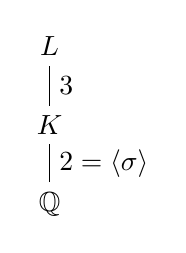
\begin{tikzpicture}
      \node (Q) {$\Q$};
      \node (K) at (0, 1) {$K$};
      \node (L) at (0, 2) {$L$};
      \draw (Q) -- (K) node [pos=0.5, right] {$2 = \bra \sigma\ket$};
      \draw (K) -- (L) node [pos=0.5, right] {$3$};
    \end{tikzpicture}
  \end{center}
  Since $L/\Q$ is unramified outside $5$ and $7$, we know that $K$ must be one of $\Q(\sqrt{5})$, $\Q(\sqrt{-7})$ and $\Q(\sqrt{-35})$. We then consider each case in turn, and then see what are the possibilities for $L$. We shall only do the case $K = \Q(\sqrt{-7})$ here. If we perform similar computations for the other cases, we find that the other choices of $K$ do not work.

  So fix $K = \Q(\sqrt{-7})$. We want $L/K$ to be cylic of degree $3$, and $\sigma$ must act non-trivially on $L$ (otherwise we get an abelian extension).

  Thus, by global class field theory, we want to find a subgroup $U \leq J_K$ of index $3$ such that $\mathcal{O}_v^\times \subseteq U$ for all $v \nmid 35$. We also need $\sigma(U) = U$, or else the composite extension would not even be Galois, and $\sigma$ has to acts as $-1$ on $J_K/U \cong \Z/3\Z$ to get a non-abelian extension.

  We know $K = \Q(\sqrt{-7})$ has has class number $1$, and the units are $\pm 1$. So we know
  \[
    \frac{C_K}{C_K^0} = \frac{\hat{\mathcal{O}}_K^\times}{\{\pm 1\}}.
  \]
  By assumption, we know $U$ contains $\prod_{v \nmid 35} \mathcal{O}_v^\times$. So we have to look at the places that divide $35$. In $\mathcal{O}_{\Q(\sqrt{-7})}$, the prime $5$ is inert and $7$ is ramified.

  Since $5$ is inert, we know $K_5/\Q_5$ is an unramified quadratic extension. So we can write
  \[
    \mathcal{O}_{(5)}^\times = \F_{25}^\times \times (1 + 5\mathcal{O}_{(5)})^\times.
  \]
  The second factor is a pro-5 group, and so it must be contained in $U$ for the quotient to have order $3$. On $\F_{25}^\times$, $\sigma$ acts as the Frobenius $\sigma(x) = x^5$. Since $\F_{25}^\times$ is cyclic of order $24$, there is a unique index $3$ subgroup, cylic of order $6$. This gives an index $3$ sugroup $U_5 \subseteq \mathcal{O}_{(5)}^\times$. Moreover, on here, $\sigma$ acts by $x \mapsto x^5 = x^{-1}$. Thus, we can take
  \[
    U = \prod_{v \not= (5)} \mathcal{O}_v^\times \times U_5,
  \]
  and this gives an $S_3$ extension of $\Q$ that is unramified outside $5$ and $7$. It is an exercise to explicitly identify this extension. % do this

  We turn to the prime $7 = -\sqrt{-7}^2$. Since this is ramified, we have
  \[
    \mathcal{O}_{(\sqrt{-7})}^\times = \F_7^\times \times \left(1 + (\sqrt{-7}) \mathcal{O}_{\sqrt{-7}}\right)^{\times},
  \]
  and again the second factor is a pro-$7$ group. Moreover $\sigma$ acts trivially on $\F_7^\times$. So $U$ must contain $\mathcal{O}_{(\sqrt{-7})}^\times$. So what we found above is the unique such extension.
\end{eg}

We previously explicitly described $C_\Q$ as $\R_{>0}^\times \times \hat{\Z}$. it would be nice to have a similar description of $C_K$ for an arbitrary $K$. The connected component will come from the infinite places $K_\infty^\times \prod_{v \mid \infty} K_v^\times$. The connected component is given by
\[
  K_\infty^{\times, 0} = (\R^\times_{> 0})^{r_1} \times (\C^\times)^{r_2},
\]
where there are $r_1$ real places and $r_2$ complex ones. Thus, we find that
\begin{prop}
  \[
    C_K/C_K^0 = \frac{\{\pm 1\}^{r_1} \times \hat{K}^\times}{\overline{K^\times}}.
  \]
\end{prop}

There is a natural map from the ideles to a more familiar group, called the content homomorphism.
\begin{defi}[Content homomorphism]\index{content homomorphism}
  The \emph{content homomorphism} is the map
  \begin{align*}
    c: J_K&\to \text{ fractional ideals of }K\\
    (x_v)_v &\mapsto \prod_{v \nmid \infty}\mathfrak{p}_v^{v(x_v)},
  \end{align*}
  where $\mathfrak{p}_v$ is the prime ideal corresponding to $v$. We ignore the infinite places completely.
\end{defi}
Observe that $c(K^\times)$ is the set of all principal ideals by definition. Moreover, the kernel of the content map is $K_\infty^\times \times \hat{\mathcal{O}}_K^\times$, by definition. So we have a short exact sequence
\[
  1 \to \frac{\{\pm 1\}^{r_1} \times \hat{\mathcal{O}}_K^\times}{\overline{\mathcal{O}_K^\times}} \to C_K /C_K^0 \to \Cl(K) \to 1.
\]
If $K = \Q $ or $\Q(\sqrt{-D})$, then $\overline{\mathcal{O}_K^\times} = \mathcal{O}_K^\times$ is finite, and in particular is closed. But in general, it will not be closed, and taking the closure is indeed needed.

Returning to the case $K = \Q$, our favorite abelian extensions are those of the form $L = \Q(\zeta_N)$ with $N > 1$. This comes with an Artin map
\[
  \hat{\Z}^\times \cong C_\Q/C_\Q^0 \to \Gal(L/\Q) \cong (\Z/N\Z)^\times.
\]
By local class field theory for $\Q_p$, we see that with our normalizations, this is just the quotient map, whose kernel is
\[
  (1 + N \hat{\Z})^\times = \prod_{p \nmid N}\Z_p^\times \times \prod_{p \mid N} (1 + N \Z_p)^\times \subseteq \prod \Z_p^\times = \hat{\Z}^\times.
\]
Note that if we used the arithmetic Frobenius, then we would get the \emph{inverse} of the quotient map.

These subgroups of $\hat{\Z}^\times$ are rather special ones. First of all $(1 + N \hat{\Z})^\times$ form a neighbourhood of the identity in $\hat{\Z}^\times$. Thus, any open subgroup contains a subgroup of this form. Equivalently, every abelian extension of $\Q$ is contained in $\Q(\zeta_N)$ for some $N$. This is the \term{Kronecker--Weber theorem}.

For a general number field $K$, we want to write down an explicit basis for open subgroups of $1$ in $\pi_0(C_k)$.
\begin{defi}[Modulus]\index{modulus}
  A \emph{modulus} is a finite formal sum
  \[
    \mathfrak{m} = \sum_{v \in \Sigma_k} m_v \cdot (v)
  \]
  of places of $K$, where $m_v \geq 0$ are integers.
\end{defi}

Given a modulus $\mathfrak{m}$, we define the subgroup
\[
  U_\mathfrak{m} = \prod_{v \mid \infty, m_v > 0}\!\! K_v^{\times, 0} \times \prod_{v \mid \infty, m_v = 0} \!\!K_v^\times \times \prod_{v \nmid \infty, m_v > 0} (1 + \mathfrak{p}_v^{m_v} \mathcal{O}_v)^{\times} \times \prod_{v \nmid \infty, m_v = 0} \mathcal{O}_v^\times \subseteq J_K.
\]
Then essentially by definition of the topology of $J_K$, any open subgroup of $J_K$ containing $K_\infty^{\times, 0}$ contains some $U_\mathfrak{m}$.

In our previous example, our moduli are all of the form
\begin{defi}[$\mathfrak{a}(\infty)$]\index{$\mathfrak{a}(\infty)$}
  If $\mathfrak{a} \lhd \mathcal{O}_K$ is an ideal, we write $\mathfrak{a}(\infty)$ for the modulus with $m_v = v(\mathfrak{a})$ for all $v \nmid \infty$, and $m_v = 1$ for all $v \mid \infty$.
\end{defi}

If $k = \Q$ and $\mathfrak{m} = (N)(\infty)$, then we simply get $U_\mathfrak{m} = \R_{>0}^\times \times (1 + N \hat{\Z})^\times$, and so
\[
  \frac{J_\Q}{\Q^\times U_\mathfrak{m}} = (\Z/n\Z)^\times,
\]
corresponding to the abelian extension $\Q(\zeta_N)$.

In general, we define
\begin{defi}[Ray class field]
  If $L/K$ is abelian with $\Gal(L/K) \cong J_K/K^\times U_\mathfrak{m}$ under the Artin map, we call $L$ the \term{ray class field} of $K$ modulo $\mathfrak{m}$.
\end{defi}

\begin{defi}[Conductor]
  If $L$ corresponds to $U \subseteq J_K$, then $U \supseteq K^\times U_\mathfrak{m}$ for some $\mathfrak{m}$. The minimal such $\mathfrak{m}$ is the \term{conductor} of $L/K$.
\end{defi}

\subsection{Ideal-theoretic description of global class field theory}
Originally, class field theory was discovered using ideals, and the ideal-theoretic formulation is at times more convenient.

Let $\mathfrak{m}$ be a modulus, and let $S$ be the set of finite $v$ such that $m_v > 0$. Let $I_S$\index{$I_S$} be the group of fractional ideals prime to $S$. Consider
\[
  P(\mathfrak{m}) = \{(x) \in I(S): x \equiv 1 \bmod {\mathfrak{m}}\}.
\]
To be precise, we require that for all $v \in S$, we have $v(x - 1) \geq m_v$, and for all infinite $v$ real with $m_v > 0$, then $\tau(x) > 0$ for $\tau: K \to \R$ the corresponding to $v$. In other words, $x \in K^\times \cap U_\mathfrak{m}$.

Note that if $\mathfrak{m}$ is trivial, then $I_S/P_\mathfrak{m}$ is the ideal class group. Thus, it makes sense to define
\begin{defi}[Ray class group]
  Let $\mathfrak{m}$ be a modulus. The \term{generalized ideal class group}, or \term{ray class group} modulo $\mathfrak{m}$ is
  \[
    \Cl_\mathfrak{m}(K) = I_S/P_\mathfrak{m}.
  \]
\end{defi}
One can show that this is always a finite group.

\begin{prop}
  There is a canonical isomorphism
  \[
    \frac{J_K}{K^\times U_\mathfrak{m}} \overset{\sim}{\to} \Cl_\mathfrak{m}(K)
  \]
  such that for $v \not \in S\cup \Sigma_{K, \infty}$, the composition
  \[
    K_v^\times \hookrightarrow J_K \to \Cl_\mathfrak{m}(K)
  \]
  sends $x \mapsto \mathfrak{p}_v^{-v(x)}$.

  Thus, in particular, the Galois group $\Gal(L/K)$ of the ray class field modulo $\mathfrak{m}$ is $\Cl_\mathfrak{m}(K)$. Concretely, if $\mathfrak{p} \not \in S$ is an ideal, then $[\mathfrak{p}] \in \Cl_{\mathfrak{m}}(K)$ corresponds to $\sigma_\mathfrak{p} \in \Gal (L/K)$, the arithmetic Frobenius. This was Artin's original reciprocity law.
\end{prop}

When $\mathfrak{m} = 0$, then this map is the inverse of the map given by content. However, in general, it is not simply (the inverse of) the prime-to-$S$ content map, even for ideles whose content is prime to $S$. According to Fr\"olich, this is the ``\term{fundamental mistake of class field theory}''.


\begin{proof}[Proof sketch]
  Let $J_K(S) \subseteq J_K$ be given by
  \[
    J_K(S) = \prod_{v \not\in S \cup \Sigma_{K, \infty}} K_v^\times.
  \]
  Here we do have the inverse of the content map
  \begin{align*}
    c^{-1}: J_K(S) &\twoheadrightarrow I_S\\
    (x_v) &\mapsto \prod \mathfrak{p}_v^{-v(x_v)}
  \end{align*}
  We want to extend it to an isomorphism. Observe that
  \[
    J_K(S) \cap U_\mathfrak{m} = \prod_{v \not \in S \cup \Sigma_{K, \infty}} \mathcal{O}_v^\times,
  \]
  which is precisely the kernel of the map $c^{-1}$. So $c^{-1}$ extends uniquely to a homomorphism
  \[
    \frac{J_K(S) U_\mathfrak{m}}{U_\mathfrak{m}} \cong \frac{J_K(S)}{J_K(S) \cap U_\mathfrak{m}} \to I_S.
  \]
  We then use that $K^\times J_K(S) U_\mathfrak{m} = J_K$ (weak approximation), and
  \[
    K^\times \cap V_\mathfrak{m} = \{x \equiv 1 \bmod{\mathfrak{m}},\; x \in K^*\},
  \]
  where
  \[
    V_\mathfrak{m} = J_K(S) U_\mathfrak{m} = \{(x_v)\in J_K \mid \text{ for all $v$ with $m_v > 0$, }x_v \in U_\mathfrak{m}\}.\qedhere
  \]
\end{proof}

\section{Hecke characters and abelian \texorpdfstring{$L$}{L}-functions}
\begin{prop}
  Let $G$ be a profinite group, and $\rho: G \to \GL_n(\C)$ continuous. Then $\ker \rho$ is open.
\end{prop}
Of course, the kernel is always closed.

\begin{proof}
  It suffices to show that $\ker \rho$ contains an open subgroup. We use the fact that $\GL_n(\C)$ has ``no small subgroups'', i.e.\ there is an open neighbourhood $U$ of $1 \in \GL_n(\C)$ such that $U$ contains no non-trivial subgroup of $\GL_n(\C)$ (exercise!). For example, if $n = 1$, then we can take $U$ to be the right half plane.

  Then for such $U$, we know $\rho^{-1}(U)$ is open. So it contains an open subgroup $V$. Then $\rho(V)$ is a subgroup of $\GL_n(\C)$ contained in $U$, hence is trivial. So $V \subseteq \ker (\rho)$.
\end{proof}

While the multiplicative group of a local field is not profinite, it is close enough, and we similarly have
\begin{ex}
  Let $F$ be a local field. Then any continuous homomorphism $F^\times \to \C^\times$ has an open kernel, i.e.\ $\chi(1 + \mathfrak{p}_F^N) = 1$ for some $N \gg 0$.
\end{ex}

We are ultimately interested in (continuous) representations of the idele group $\chi: J_K \to \C^\times$. While $J_K$ is not profinite, it contains the group $\hat{\mathcal{O}}_K^\times$ which \emph{is} profinite. Thus, $\ker \chi$ contains an open subgroup of $\hat{\mathcal{O}}_K^\times$. 

In particular, if also $\chi(K_\infty^{\times, 0}) = 1$, then $\chi$ has finite image.

We say $\chi$ is unramified if $\chi|_{\mathcal{O}_F^\times} = 1$.
\begin{ex}
  $\chi$ is unramified iff $\chi(x) = |x|_F^s$ for some $s \in \C$.
\end{ex}

If $F \cong \R$, we say $\chi: F^\times \to \C^\times$ is unramified if $\chi(-1) = 1$ (so $\chi(x) = |x|^s$ for some $s$).

Going back to global fields, we have
\begin{prop}
  The set of continuous homomorphisms $\chi: J_K = \prod_v' K_v^\times \to \C^\times$ bijects with the set of all families $(\chi_v)_{v \in \Sigma_k}$, $\chi_v: K_v^\times \to \C^\times$ such that $\chi_v$ is unramified for almost all (i.e.\ all but finitely many) $v$, with the bijection given by $\chi \mapsto (\chi_v)$, $\chi_v = \chi|_{K_v^\times}$.
\end{prop}

\begin{proof}
  Given $\chi$, we know $\chi(\hat{\mathcal{O}}_K^\times)$ is finite. So $\chi(\mathcal{O}_v^\times) = 1$ for almost all finite $v$. So we have a map from the LHS to the RHS. As
  \[
    \bigoplus_{v \not \in \Sigma_{K, \infty}} \mathcal{O}_v^\times \subseteq \prod_{v \nmid \infty} \mathcal{O}_v^\times
  \]
  is dense, we know $\bigoplus_v K_v^\times \subseteq J_K$ is dense, and so this map is an inclusion.

  Finally, let $(\chi_v)_v$ be an element of the RHS. So by the hypothesis,
  \[
    \prod_{v \nmid \infty} (\ker \chi_V \cap \mathcal{O}_v^\times) \subseteq \hat{K}^\times
  \]
  is open. So the map $\chi^\infty: \hat{K}^\times \to \C^\times$ given by $(x_v)_{v \nmid \infty} \mapsto \prod \chi_v(x_v)$ is well-defined. So we define
  \[
    \chi = \chi_\infty \chi^\infty,\quad \chi_\infty = \prod_{v \mid \infty} \chi_v: K_\infty^\times \to \C^\times.\qedhere
  \]
\end{proof}

\begin{defi}[Hecke character]\index{Hecke character}
  A \emph{Hecke character} is a continuous (not necessarily unitary) homomorphism
  \[
    \chi: J_K/K^\times \to \C^\times.
  \]
\end{defi}
These are also known as \term{quasi-characters} in some places, where character means unitary. However, we shall adopt the convention that characters need not be unitary.

By what we have just said, we can write $\chi = \chi_\infty \chi^\infty$, where $\chi_\infty: K_\infty^\times \to \C^\times$, and $\chi^\infty: \hat{K}^\times \to \C^\times$.

\begin{eg}
  $\chi$ has finite order iff $\chi(C_K^0) = 1$ iff $\chi_\infty(K_\infty^{\times, 0}) = 1$, iff $\chi_\infty^2 = 1$, iff $\chi$ factors through $\Cl_\mathfrak{m}(K)$ for some modulus $\mathfrak{m}$. We say $\chi$ is a \term{ray class character}.
\end{eg}

\begin{eg}
  The idele norm $\|\ph\|_{\A}: C_K \to \R^\times_{>0}$ is a character not of finite order. In the case $K = \Q$, we have $C_\Q = \R_{>0}^\times \times \hat{\Z}^\times$. The idele norm is then the first projection onto $\R_{>0}^\times$. So the Hecke characters of $C_\Q$ are all of the form
  \[
    \chi(x) = |x|_{\A}^s \cdot \chi'(x),
  \]
  where $\chi'$ has finite order, i.e.\ is a Dirichlet character
  \[
    C_\Q \to \hat{\Z}^\times \to (\Z/N\Z)^\times \to \C^\times
  \]
  for some $N$.
\end{eg}
For other fields, there can be more interesting Hecke characters.

For a general field $K$, we have finite order characters as we just saw. They correspond to characters on $I_S$ which are trivial on $P_\mathfrak{m}$. In fact, we can describe all Hecke characters in terms of ideals.

\subsection{Ideal-theoretic description of any Hecke character}
Choose a modulus $\mathfrak{m}$ such that $\chi^\infty$ is trivial on $\hat{K}^\times \cap U_\mathfrak{m}$. Let $S$ be the set of finite $v$ such that $\mathfrak{m}_v$ is positive. Define a homomorphism $\Theta: I_S \to \C^\times$ as follows: if $v \not \in S$, so that $\chi_v(\mathcal{O}_v^\times) = 1$, send
\[
  \mathfrak{p}_v \mapsto \chi_v(\pi_v)^{-1}.
\]
If this were a Hecke character of finite order, then this would be trivial on $P_\mathfrak{m}$. Let $x \in K^\times$ with $x \equiv 1 \bmod{\mathfrak{m}}$. Then for all $v \in S$, we have $\chi_v(x) = 1$. So
\[
  1 = \chi(x) = \chi_\infty(x) \prod_{v \not \in S\text{ finite}} \chi_v(x) = \chi_\infty(x) \prod_{\text{finite }v \not \in S} \chi_v(\pi_v)^{v(x)}.
\]
So by definition of $\Theta$, we have
\[
  \chi_\infty(x) = \Theta(x).
\]
In other words, we get a map
\begin{multline*}
  \Hom_{cts}(C_K, \C^\times) \to \{(\Theta, \mathfrak{m}) : \Theta: I_S \to \C^\times, \;x \equiv 1 \pmod {\mathfrak{m}} \Rightarrow \Theta(x) \\
  = \chi_\infty(x)\text{ for some}\chi_\infty: K_\infty^\times \to \C^\times\}/\sim
\end{multline*}
where we quotient out by what happens when we change modulus.

It is not hard to see that this is in fact a bijection. This is Hecke's original definition of his Gr\"o{\ss}encharakter.

What do general Hecke characters have to do with Galois groups?
\begin{eg}
  Let $K = \Q(i) \subseteq \C$. Let
  \[
    \mathfrak{m} = 3 (v_2),
  \]
  where $v_2$ is a place over $2$, corresponding to $(1 + i) \mathcal{O}_K$. What is special about this modulus is that we in fact have
  \[
    \mathcal{O}_{v_2}^\times = (1 + (1 + i)^3 \mathcal{O}_v) \times \mu_4.
  \]

  Of course, $\Cl(K) = 1$, so
  \[
    C_K = \frac{\C^\times \times \hat{\mathcal{O}}_K^\times}{\mu_4 = \{\pm 1, \pm i\}}.
  \]
  To write down characters of $C_K$, observe that we have a surjection
  \[
    \hat{\mathcal{O}}_K^\times \twoheadrightarrow \mathcal{O}_{v_2}^\times = (1 + (1 + i)^3 \mathcal{O}_v) \times \mu_4
  \]
  since
  \[
    \left(\frac{\Z[i]}{(2 + 2i)}\right)^\times = \{\pm 1, \pm i\}.
  \]
  Cancelling the $\mu_4$, there is a unique $\chi: C_K \to \C^\times$ that is trivial on
  \[
    \prod_{v \not \in \{v_2, \infty\}} \mathcal{O}_v^\times \times (1 + (1 + i)^3 \mathcal{O}_{v_2}),
  \]
  such that $\chi_\infty(z) = z$. This is a Hecke character not of the form we have had before.

  We can say what this is in ideal-theoretic terms. If $\mathfrak{p} \not= (1 + i)$ is a prime ideal of $K$, then $\mathfrak{p} = (\pi)$ for $\pi \equiv 1 \bmod (2 + 2i)$ for a unique $\pi = \pi_\mathfrak{p}$. The associated $\Theta: I_{\{v_2\}} \to \C^\times$ is just given by $\Theta(\mathfrak{p}) = \pi_\mathfrak{p}$.

  This is an example of an algebraic Hecke character.
\end{eg}

\begin{defi}[Algebraic homomorphism]\index{algebraic homomorphism}
  A homomorphism $K^\times \to \C^\times$ is \emph{algebraic} if there exists integers $n(\sigma)$ (for all $\sigma: K \hookrightarrow \C$) such that
  \[
    \varphi(x) = \prod \sigma(x)^{n(\sigma)}.
  \]
\end{defi}
The first thing to note is that if $\varphi$ is algebraic, then $\varphi(K^\times)$ is contained in the Galois closure of $K$ in $\C$. In particular, it takes values in the number field. Another equivalent definition is that it is algebraic in the sense of algebraic geometry, i.e.\ if $K = \bigoplus \Q e_i$ for $i = 1, \ldots, n$ as a vector space, then we can view $K$ as the $\Q$-points of an $n$-dimensional affine group scheme. We can then define $R_{K/\Q} \G_m \subseteq \A$ to be the set on which $X$ is invertible, and then an algebraic Hecke character is a homomorphism of algebraic groups $(T_K)/\C \to \G_m/\C$, where $T_K = \Res_{K/\Q}(\G_m)$.

If we have a real place $v$ of $K$, then this corresponds to a real embedding $\sigma_v: K \to K_v \cong \R$, and if $v$ is a complex place, we have a pair of embedding $\sigma_v, \bar{\sigma}_v: K \hookrightarrow K_v \simeq \C$, picking one of the pair to be $\sigma_v$. So $\varphi$ extends to a homomorphism
\[
  \varphi: K_\infty^\times \to \C^\times
\]
given by
\[
  \varphi(x_v) = \prod_{v\text{ real}} x_v^{n(\sigma_v)} \prod_{v\text{ complex}} x_v^{n(\sigma_v)} \bar{x}_v^{n(\bar{\sigma}_v)}
\]
\begin{defi}[Algebraic Hecke character]\index{algebraic Hecke character}
  A Hecke character $\chi = \chi_\infty \chi^\infty: J_K/K^\times \to \C^\times$ is \emph{algebraic} if there exists an algebraic homomorphism $\varphi: K^\times \to \C^\times$ such that $\varphi(x) = \chi_\infty(x)$ for all $x \in K_\infty^{\times, 0}$, i.e.\ $\chi_\infty = \varphi \prod_{v\text{ real}} \sgn_v^{e_v}$ for $e_v \in \{0, 1\}$.

  We say $\varphi$ (or the tuple $(n(\sigma))_\sigma$) is the \term{infinite type} of $\chi$.
\end{defi}
\begin{eg}
  The adelic norm $|\ph|_{\A}: J_K \to \C^\times$ has
  \[
    \chi_\infty = \prod |\ph|_v,
  \]
  and so $\chi$ is algebraic, and the associated $\varphi$ is just $N_{K/\Q}: K^\times \to \Q^\times \subseteq \C^\times$, with $(n_\sigma) = (1, \ldots, 1)$. 
\end{eg}

\begin{ex}
  Let $K = \Q(i)$, and $\chi$ from the previous example, whose associated character of ideals was $\Theta: \mathfrak{p} \mapsto \pi_\mathfrak{p}$, where $\pi_\mathfrak{p} \equiv 1 \pmod (2 + 2i)$. The infinity type is the inclusion $K^\times \hookrightarrow \C^\times$, i.e.\ it has type $(1, 0)$.
\end{ex}

Observe that the image of an algebraic homomorphism $\varphi: K^\times \to \C^\times$ lies in the normal closure of $K$. More generally,
\begin{prop}
  If $\chi$ is an algebraic Hecke character, then $\chi^\infty$ takes values in some number field. We write $E = E(\chi)$ for the smallest such field.
\end{prop}
Of course, we cannot expect $\chi$ to take algebraic values, since $J_K$ contains copies of $\R$ and $\C$.

\begin{proof}
  Observe that $\chi^\infty(\hat{\mathcal{O}}_K^\times)$ is finite subgroup, so is $\mu_n$ for some $n$. Let $x \in K^\times$, totally positive. Then
  \[
    \chi^\infty(x) = \chi_\infty(x)^{-1} = \varphi(x)^{-1} \in K^{cl},
  \]
  where $K^{cl}$ is the Galois closure. Then since $K_{>0}^\times \times \hat{\mathcal{O}}_K^\times \to \hat{K}^\times$ has finite cokernel (by the finiteness of the class group), so
  \[
    \chi^\infty(\hat{K}^\times) = \coprod_{i = 1}^d z_i \chi^\infty(K_{>0}^\times  \hat{\mathcal{O}}_K^\times),
  \]
  where $z_i^d  \in \chi^\infty(K_{>0}^\times \hat{\mathcal{O}}_K^\times)$, and is therefore contained inside a finite extension of the image of $K_{>0}^\times \times \hat{\mathcal{O}}_K^\times$.
\end{proof}

Hecke characters of finite order (i.e.\ algebraic Hecke characters with infinity type $(0, \ldots, 0)$) are in bijection with continuous homomorphisms $\Gamma_K \to \C^\times$, necessarily of finite order. What we show now is how to associate to a general algebraic Hecke character $\chi$ a continuous homomorphism $\psi_\ell: \Gamma_K \to E(\chi)_\lambda^\times \supseteq \Q_\ell^\times$, where $\lambda$ is a place of $E(X)$ over $\ell$. This is continuous for the $\ell$-adic topology on $E_\lambda$. In general, this will not be of finite order. Thus, algebraic Hecke characters correspond to $\ell$-adic Galois representations.

The construction works as follows: since $\chi^\infty(x) = \varphi(x)^{-1}$, we can restrict the infinity type $\varphi$ to a homomorphism $\varphi: K^\times \to E^\times$. We define $\tilde{\chi}: J_K \to E^\times$ as follows: if $x = x_\infty x^\infty \in K_\infty^\times K^{\infty, \times} \in J_K$, then we set
\[
  \tilde{\chi}(x) = \chi(x) \varphi(x_\infty)^{-1}.
\]
Notice that this is not trivial on $K^\times$ in general. Then $\tilde{\chi}_\infty$ takes values in $\{\pm 1\}$. Thus, $\tilde{\chi}$ takes values in $E^\times$. Thus, we know that $\tilde{\chi}$ has open kernel, i.e.\ it is continuous for the discrete topology on $E^\times$, and $\tilde{\chi}|_{K^\times} = \varphi^{-1}$.

Conversely, if $\tilde{\chi}: K^\times \to E^\times$ is a continuous homomorphism for the discrete topology on $E^\times$, and $\tilde{\chi}|_{K^\times}$ is an algebraic homomorphism, then it comes from an algebraic Hecke character in this way.

Let $\lambda$ be a finite place of $E$ over $\ell$, a rational prime. Recall that $\varphi: K^\times \to E^\times$ is an algebraic homomorphism, i.e.
\[
  \varphi\left(\sum x_i e_i\right) = f(\mathbf{x}),\quad f \in E(X_1, \ldots, X_n).
\]
We can extend this to $K_\ell^\times = (K \otimes_{\Q} \Q_\ell)^\times = \prod_{v \mid \ell} K_v^\times$ to get a homomorphism
\[
  \varphi_\lambda: K_\ell^\times \to E_\lambda^\times
\]
This is still algebraic, so it is certainly continuous for the $\ell$-adic topology.

Now consider the character $\psi_\lambda: J_K \to E_\lambda^\times$, where now
\[
  \psi_\lambda((x_v)) = \tilde{\chi}(x) \varphi_\lambda((x_v)_{v \mid \ell}).
\]
This is then continuous for the $\ell$-adic topology on $E_\lambda^\times$, and moreover, we see that $\psi_\lambda(K^\times) = \{1\}$ as $\tilde{\chi}|_{K^\times} = \varphi^{-1}$ while $\varphi_\lambda|_{K^\times} = \varphi$.  Since $\tilde{\chi}(K_\infty^{\times, 0}) = \{1\}$, we know that $\psi_\lambda$ it is in fact defined on $C_K/C_K^0 \cong \Gamma_K^{ab}$.

Obviously, $\psi_\lambda$ determines $\tilde{\chi}$ and hence $\chi$. 
\begin{fact}
  An $\ell$-adic character $\psi: C_K/C_K^0 \to E_\lambda^\times$ comes from an algebraic Hecke character in this way if and only if the associated Galois representation is \emph{Hodge--Tate}, which is a condition on the restriction to the decomposition groups $\Gal(\bar{K}_v/K_v)$ for the primes $v \mid \ell$.
\end{fact}

\begin{eg}
  Let $K = \Q$ and $\chi = |\ph |_{\A}$, then
  \[
    \tilde{\chi} = \sgn(x_\infty) \prod_p |x_p|_p.
  \]
  So
  \[
    \psi_\ell((x_v)) = \sgn(x_\infty) \prod_{p \not= \ell} |x_p|_p \cdot |x_\ell|_{\ell} \cdot x_\ell.
  \]
  Note that $|x_\ell|_{\ell} x_\ell \in \Z_\ell^\times$. We have
  \[
    C_\Q/C_\Q^0 \cong \hat{\Z}^\times.
  \]
  Under this isomorphism, the map $\hat{\Z}^\times \Q_\ell^\times$ is just the projection onto $\Z_\ell^\times$ followed by the inclusion, and by class field theory, $\psi_\ell: \Gal(\bar{\Q}/\Q) \to \Z_\ell^\times$ is just the cyclotomic character of the field $\Q(\{\zeta_{\ell^n}\})$,
  \[
    \sigma(\zeta_{\ell^n}) = \zeta_{\ell^n} ^{\psi_\ell(\sigma) \bmod \ell^n}.
  \]
\end{eg}

\begin{eg}
  Consider the elliptic curve $y^2 = x^3 - x$ with complex multiplication over $\Q(i)$. In other words, $\End(E/\Q(i)) = \Z[i]$, where we let $i$ act by
  \[
    i \cdot (x, y) \mapsto (-x, iy).
  \]
  Its Tate module
  \[
    T_\ell E = \lim \E[\ell^n]
  \]
  is a $\Z_\ell [i]$-module. If $\lambda \mid \ell$, then we define
  \[
    V_\lambda E = T_\ell E \otimes_{\Z_{\ell}[i]} K_\lambda.
  \]
  Then $\Gamma_K$ act by $\Gamma_K: \Aut_{K_\lambda} V_\lambda E = K_\lambda^\times$.
\end{eg}

We now want to study the infinity types of an algebraic Hecke character.
\begin{lemma}
  Let $K$ be a number field, $\varphi: K^\times \to E^\times \subseteq \C^\times$ be an alegbraic homomorphism, and suppose $E/\Q$ is Galois. Then $\varphi$ factors as
  \[
    K^\times \overset{\mathrm{norm}}{\longrightarrow} (K \cap E)^\times \overset{\phi'}{\longrightarrow} E^\times.
  \]
  Note that since $E$ is Galois, the intersection $K \cap E$ makes perfect sense.
\end{lemma}

\begin{proof}
  By definition, we can write
  \[
    \varphi(x) = \prod_{\sigma : K \hookrightarrow \C} \sigma(x)^{n(\sigma)}.
  \]
  Then since $\varphi(x) \in E$, for all $x \in K^\times$ and $\tau \in \Gamma_E$, we have
  \[
    \prod \tau \sigma(x) ^{n(\sigma)} = \prod \sigma(x)^{n(\sigma)}.
  \]
  In other wrods, we have
  \[
    \prod_\sigma \sigma(x)^{n(\tau^{-1} \sigma)} = \prod_\sigma \sigma(x)^{n(\sigma)}.
  \]
  Since the homomorphisms $\sigma$ are independent, we must have $n(\tau \sigma) = n (\sigma)$ for all embeddings $\sigma: K \hookrightarrow \bar{\Q}$ and $\tau \in \Gamma_E$. This implies the theorem.
\end{proof}

Recall that if $\mathfrak{m}$ is a modulus, then we defined open subgroups $U_\mathfrak{m} \subseteq J_K$, consisting of the elements $(x_v)$ such that if a real $v \mid \mathfrak{m}$, then $x_v > 0$, and if $v \mid \mathfrak{m}$ for a finite $v$, then $v(x_v - 1) \geq m_v$. We can write this as
\[
  U_\mathfrak{m} = U_{\mathfrak{m}, \infty} \times U_{\mathfrak{m}}^\infty.
\]
\begin{prop}
  Let $\varphi: K^\times \to \C^\times$ be an algebriac homomorphism. Then $\varphi$ is the infinity type of an algebraic Hecke character $\chi$ iff $\varphi(\mathcal{O}_K^\times)$ is finite.
\end{prop}

\begin{proof}
  To prove the $(\Rightarrow)$ direction, suppose $\chi = \chi_\infty \chi^\infty$ is an algebraic Hecke character with infinity type $\varphi$. then $\chi^\infty(U_\mathfrak{m}^\infty) = 1$ for some $\mathfrak{m}$. Let $E_\mathfrak{m} = K^\times \cap U_\mathfrak{m} \subseteq \mathcal{O}_K^\times$, a subgroup of finite index. As $\chi^\infty(E_\mathfrak{m}) = 1 = \chi(E_\mathfrak{m})$, we know $\chi_\infty(E_\mathfrak{m}) = 1$. So $\varphi(\mathcal{O}_K^\times)$ is finite.

  To prove $(\Leftarrow)$, given $\varphi$ with $\varphi(\mathcal{O}_K^\times)$ finite, we can find some $\mathfrak{m}$ such that $\varphi(E_\mathfrak{m}) = 1$. Then $(\varphi, 1): K_\infty^\times \times U_\mathfrak{m}^\infty \to \C^\times$ is trivial on $E_\mathfrak{m}$. So we can extend this to a homomorphsim
  \[
    \frac{K_\infty^\times U_\mathfrak{m} K^\times}{K^\times} \cong \frac{K_\infty^\times U_\mathfrak{m}}{E_\mathfrak{m}} \to \C^\times,
  \]
  since $E_\mathfrak{m} = K^\times \cap U_\mathfrak{m}$. But the LHS is a finite index subgroup of $C_K$. So the map extends to some $\chi$.
\end{proof}

Here are some non-standard terminology:
\begin{defi}[Serre type]\index{Serre type}
  A homomorphism $\varphi: K^\times \to \C^\times$ is of \emph{Serre type} if it is algebraic and $\varphi(\mathcal{O}_K^\times)$ is finite.
\end{defi}
These are precisely homomorphisms that occur as infinity types of algebraic Hecke characters.

Note that the unit theorem implies that
\[
  \mathcal{O}_K^\times \hookrightarrow K_\infty^{\times, 1} = \{x \in K_\infty^{\times} : |x|_{\A} = 1\}
\]
has compact cokernel. If $\varphi(\mathcal{O}_K^\times)$ is finite, then $\varphi(K_\infty^{\times, 1})$ is compact. So it maps into $\U(1)$.

\begin{eg}
  Suppose $K$ is totally real. Then
  \[
    K_\infty^\times = (\R^\times)^{\{\sigma: K \hookrightarrow \R\}}.
  \]
  Then we have
  \[
    K_\infty^{\times, 1} = \{(x_\sigma): \prod x_\sigma = \pm 1\}.
  \]
  Then $\varphi((x_\sigma)) = \prod x_\sigma^{n(\sigma)}$, so $|\varphi(K_\infty^{\times, 1})| = 1$. In other words, all the $n_\sigma$ are equal. Thus, $\varphi$ is just a power of the norm map.

  Thus, algebraic Hecke characters are all of the form $|\ph |_\A^m \cdot (\text{finite order character})$.
\end{eg}

Another class of examples comes from CM fields.
\begin{defi}[CM field]\index{CM field}
  $K$ is a CM field if $K$ is a totally complex quadratic extension of a totally real number field $K^+$.
\end{defi}
This CM refers to \emph{complex multiplication}.

This is a rather restrictive condition, since this implies $\Gal(K/K^+) = \{1, c\} = \Gal(K_w /K_v^+)$ for every $w \mid v \mid \infty$. So $c$ is equal to complex conjugation for \emph{every} embedding $K \hookrightarrow \C$.

From this, it is easy to see that CM fields are all contained in $\Q^{CM} \subseteq \bar{\Q} \subseteq \C$, given by the fixed field of the subgroup
\[
  \bra c \sigma c \sigma^{-1}: \sigma \in \Gamma_\Q\ket \subseteq \Gamma_\Q.
\]
For example, we see that the compositum of two CM fields is another CM field.

\begin{ex}
  Let $K$ be a totally complex $S_3$-extension over $\Q$. Then $K$ is not CM, but the quadratic subfields is complex and is equal to $K \cap \Q^{CM}$.
\end{ex}

\begin{eg}
  Let $K$ be a CM field of degree $2r$. Then Dirichelt's unit theorem tells us
  \[
    \rk \mathcal{O}_K^\times = r - 1 = \rk \mathcal{O}_{K^+}^\times.
  \]
  So $\mathcal{O}_K^\times$ is a finite index subgroup of $\mathcal{O}_{K^+}^\times$. So $\varphi: K^\times \to \C^\times$ is of Serre type iff it is algebraic and its restriction to $K^{+, \times}$ is of Serre type. In other words, we need $n(\sigma) + n(\bar{\sigma})$ to be independent of $\sigma$.
\end{eg}

\begin{thm}
  Suppose $K$ is arbitrary, and $\varphi: K^\times \to E^\times \subseteq \C^\times$ is algebraic, and we assume $E/\Q$ is Galois, containing the normal closure of $K$. Thus, we can write
  \[
    \varphi(x) = \prod_{\sigma: K \hookrightarrow E} \sigma(x)^{n(\sigma)}.
  \]
  Then the following are equivalent:
  \begin{enumerate}
    \item $\varphi$ is of Serre type
    \item $\varphi = \psi \circ N_{K/F}$, where $F$ is the maximal CM subfield and $\psi$ is of Serre type
    \item For all $c' \in \Gal(E/\Q)$ conjugate to $c$, the map $\sigma \mapsto n(\sigma) + n (c' \sigma)$ is constant.
    \item (in the case $K \subseteq \C$ and $K/\Q$ is Galois with Galois group $G$) Let $\lambda = \sum n(\sigma) \sigma \in \Z[G]$. Then for all $\tau \in G$, we have
      \[
        (\tau - 1)(c + 1) \lambda = 0 = (c + 1)(\tau - 1) \lambda.
      \]
  \end{enumerate}
\end{thm}

\begin{proof}
  \begin{itemize}
    \item (iii) $\Leftrightarrow$ (iv): This is just some formal symbol manipulation.
    \item (ii) $\Rightarrow$ (i): The norm takes units to units.
    \item \qedhere
  \end{itemize}
\end{proof}
\printindex
\end{document}
